\section{ Desarrollo del cálculo de la fuerza de torsión en las palas de una turbina}

\subsection{Descripción de la pala del aerogenerador y sus parámetros}

\textcolor{orange}{\huge El punto 2.1 debería ser lo que es una turbina, sus partes (torre, góndola, rotor con palas, etc), quizás una imagen, y decir que vas a trabajar con palas, etc. Es decir, una introducción de lo que vas a desarrollar, fuerza de torsión en qué sistema y en qué parte, etc.}

En esta sección se va a describir la pala del aerogenerador y los parámetros necesarios para determinar los efectos que produce la torsión en nuestra obtención de energía. En primer lugar la definición e idea general de la pala de una turbina de un aerogenerador, después el desarrollo trigonométrico para el cálculo de la línea de cuerda y por último la obtención de los brazos de la pala conociendo los centro de masa de los segmentos.\\


Se determina que la pala de la turbina eólica es un \textbf{trapecio} cuya representación simplificada se muestra en la Figura \ref{fig:pala_simp}. \\\\

\begin{figure}[H]
    \centering
    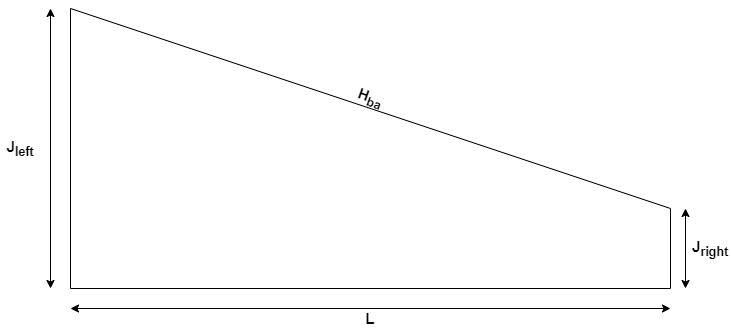
\includegraphics[width=1\textwidth]{images/pala simple.drawio.png}
    \caption{Representación de una pala de turbina eólica}
    \label{fig:pala_simp}
\end{figure}


Lo siguiente que debe tenerse presente es que se necesita también una representación de la pala como la que se puede observar en la Figura \ref{fig:pala_simp}. Esta está dividida en segmentos de igual largo para poder comprender el desarrollo que se realizará simulando una torsión, en la cual se girarán los segmentos un cierto ángulo los unos de los otros.

\begin{figure}[H]
    \centering
    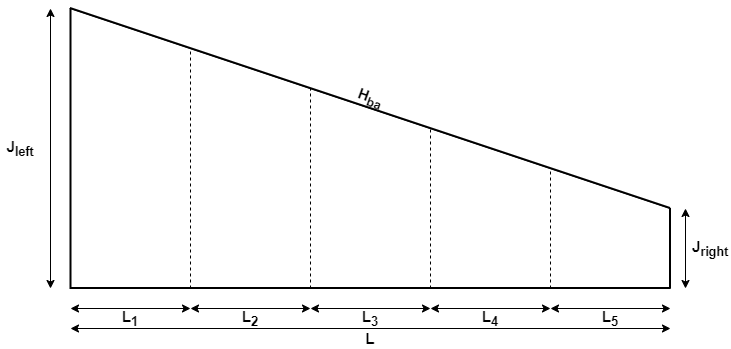
\includegraphics[width=1\textwidth]{images/pala simple segmentada.png}
    \caption{Representación de una pala de turbina eólica dividida en segmentos}
    \label{fig:pala_dividida}
\end{figure}

Por simplicidad, la pala se dividirá únicamente en $N$ segmentos, en este trabajo se utilizará $N=5$. Aunque se mantenga este valor durante el trabajo se asociará a una variable en caso de que se quieran hacer pruebas mediante simulación en MATLAB más adelante. \\
    

Se define la variable $L$ como la longitud de la pala (ver Figura \ref{fig:pala_simp}). Como puede observarse, cada uno de los segmentos de la Figura \ref{fig:pala_dividida} tendrá una longitud de segmento $L_i = \dfrac{L}{N} (m)$ donde $i \in \{1,...,N\}$.\\

Como se puede observar en la Figura \ref{fig:pala_dividida} cada segmento tiene una altura variable, esto se debe a la forma real de las palas, cuanto más cerca del buje de la turbina, mayor es el área del segmento. La altura en el centro de estos segmentos, conocida como \textit{chord line} (que se denotará como $c_i$ con $i \in \{1, ...,N\}$) o línea de cuerda, se determinará fijando los valores de la longitud de la pala $L$, la longitud del buje (que se denotará por $J_{left}$) y la longitud de la punta (que se denotará por $J_{right}$). Una vez establecidos estos valores se puede dar paso al desarrollo matemático de la pala.\\

\begin{figure}[H]
    \centering
    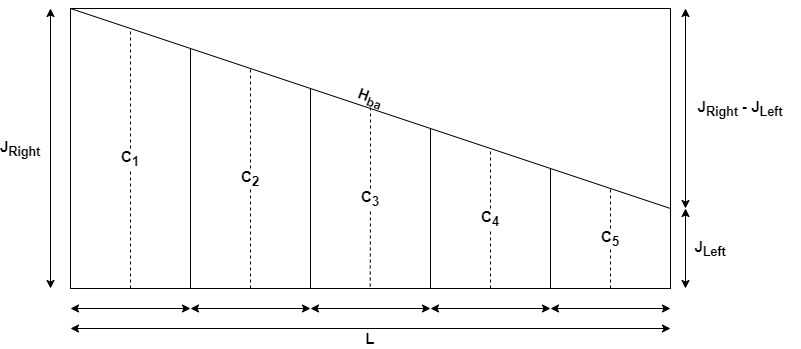
\includegraphics[width=1\textwidth]{images/planteo chord line.drawio.png}
    \caption{Representación parametrizada de la pala de una turbina eólica}
    
    \label{fig:pala_desarrollo_chord}
\end{figure}

Para el cálculo de la línea de cuerda se requiere la realización de un desarrollo trigonométrico. \\

En base a la Figura \ref{fig:pala_desarrollo_chord} se puede deducir que
$J_{rigth} = \dfrac{J_{left}}{D} (m)$ donde D es el factor de reducción de alto de pala y $D \in \mathbb{Q+}$. Además, se debe cumplir que $J_{left} > D$.\\

El factor reductor $D$ procede de la naturaleza del análisis y cómo se ha afrontado el estudio simplificado de una pala de aerogenerador. Si bien es cierto que se pudo realizar de una manera aún más simple haciendo que la pala fuese un rectángulo, se prefirió abordar con una forma trapezoidal. Así, los tres parámetros $J_{left}$, $J_{rigth}$ y $L$ se calculan en función del valor de $D$. Esto permite hacer los cálculos con una relación entre la longitud del buje $J_{left}$ y de la punta $J_{right}$ de las palas de la turbina eólica, esto además permite que el problema sea más general. \\

Se define el valor de la hipotenusa del borde de arrastre $H_{ba}$ mediante el Teorema de Pitágoras, ya que se trata de un triángulo rectángulo (en azul en la Figura \ref{fig:pala_calculo_phi}). Así, se tiene:
\begin{equation}
H_{ba} = \sqrt{(J_{left} - J_{right})^{2} + L^{2}}
\label{def_hipotenusa_pala}
\end{equation}


\begin{figure}[H]
    \centering
    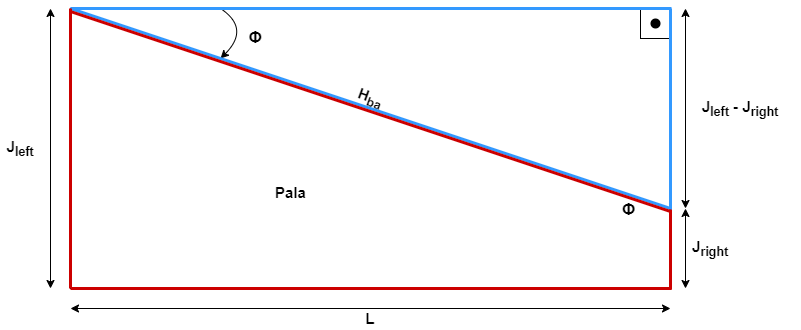
\includegraphics[width=0.9\textwidth]{images/triangulo sacar phi.png}
    \caption{Pala de la turbina en amarillo y triángulo usado para el cálculo de $\Phi$ en azul}
    
    \label{fig:pala_calculo_phi}
\end{figure}

A continuación, se debe obtener el ángulo de la línea del borde de arrastre de la pala de la turbina eólica $\Phi$, para así conocer cómo decrece el valor de $H_{ba}$.
En base a la Figura \ref{fig:pala_calculo_phi} se puede calcular de tres formas distintas mediante la trigonometría el valor del ángulo $\Phi$:
\begin{equation}
 \Phi = \arcsin{\left(\dfrac{c_{left} - c_{right}}{H_{ba}}\right)} (^{\circ})
\label{def_angulo_phi_1}
\end{equation}

\begin{equation}
 \Phi = \arccos{\left(\dfrac{L}{H_{ba}}\right)} (^{\circ})
\label{def_angulo_phi_2}
\end{equation}

\begin{equation}
 \Phi = \arctan{\left(\dfrac{\sin{\left(\dfrac{c_{left} - c_{right}}{H_{ba}}\right)}}{\cos{\left(\dfrac{L}{H_{ba}}\right)}}\right)} (^{\circ}) 
\label{def_angulo_phi_3}
\end{equation}


Para calcular las \textit{líneas de cuerda} $c$, se aíslan los trapecios más pequeños de los que se han obtenido todos los datos menos el valor de su base menor, que se tendrá que calcular, siendo este equivalente a $c$.\\

Las variables necesarias para el cálculo de las líneas de cuerda son:
\begin{equation}
 altura_i = \dfrac{(2i - 1) \cdot L}{2N} \hspace{7pt} (m)
\label{def_variables_fragmentadas1}
\end{equation}
\begin{equation}
     diagonal_i = \dfrac{(2i - 1) \cdot H_{bf}}{2N} \hspace{7pt} (m)
\label{def_variables_fragmentadas2}
\end{equation}
Donde $altura_i$ es la longitud de la pala fragmentada para el cálculo de la línea de cuerda y $diagonal_i$ es la longitud de la hipotenusa del borde de fuga fragmentada para el cálculo de la línea de cuerda.\\

Por último, una vez definido todo lo necesario, se pasa al cálculo mediante el cual se obtiene el valor de todas y cada una de las $líneas \text{ } de \text{ } cuerda$ de la pala con la que se está trabajando.\\

Primero se obtiene la diferencia mediante Pitágoras entre la base mayor y la menor, definida como $x_i$, después la resta de la base mayor y esta diferencia.
\begin{equation}
 x_i = \sqrt{diagonal_i^{2} - altura_i^{2}} \hspace{7pt} (m)
 \end{equation}
 \begin{equation}
 c_i = c_{left_i} - x_i \hspace{7pt} (m)
\label{def:chord_line}
\end{equation}

La Figura \ref{fig:sacar_c3} se ilustra un ejemplo en el que  el valor de $i$ es igual a tres, obteniendo así $c_3$. En verde el trapecio y en magenta el triángulo del que restamos el cateto a la base mayor del trapecio.\\

\begin{figure}[H]
    \centering
    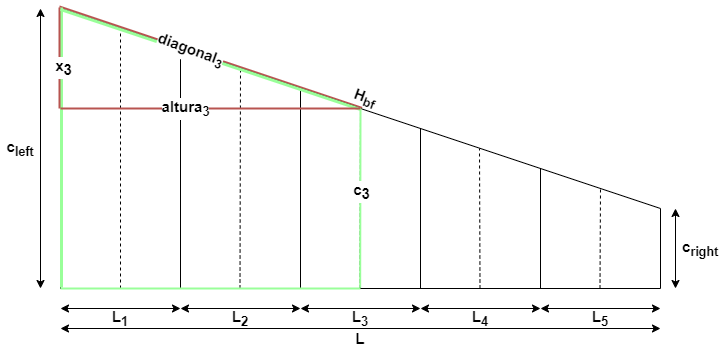
\includegraphics[width=0.9\textwidth]{images/Trapecio calculo x.png}
    \caption{Representación gráfica del cálculo de $c_3$} 
    \label{fig:sacar_c3}
\end{figure}


Una vez se ha obtenido el valor buscado, $c_i$, se deberá definir todos los laterales de los segmentos de la pala, para así poder operar con ellos y conseguir el área de cada uno. Esto ya fue desarrollado en el artículo \cite{armenta2021predictive}, pero en aquel caso fue usado para comprobar el error que suponía usar un rectángulo en vez de una pala simplificada. En este caso se parte directamente de la pala simplificada para evitar correcciones de errores mas adelante y porque el cálculo que se debe realizar con respecto a la obtención de energía como en el Artículo \cite{armenta2021predictive}.\\

En base a esta representación esquemática, y mediante las relaciones trigonométricas anteriores se obtuvieron:
\begin{equation}
 c_{left_i} = c_i + (\dfrac{L_i}{2}) \tan \varPhi \hspace{7pt} (m)
 \label{def:laterales_segmento_left}
\end{equation}
\begin{equation}
 c_{right_i} = c_i - (\dfrac{L_i}{2}) \tan \varPhi \hspace{7pt} (m)
\label{def:laterales_segmento_right}
\end{equation}

Al igual que se deduce en el artículo \cite{armenta2021predictive}, con los datos obtenidos de los laterales de cada segmento, se puede trabajar con una forma de trapecio y encontrar el área de los segmentos que se definieron en la Figura \ref{fig:pala_dividida}.\\

Aparte, con esta definición  de la Figura \ref{fig:pala_desarrollo_chord}, los valores de $c_{left_i}$ y de $c_{right_i}$ serían equivalentes a $c_{left_1}$ y a $c_{right_5}$, respectivamente. Estos son definidos a priori debido a su importancia para caracterizar la pala de manera correcta y con las dimensiones que el usuario desee.\\

Se determina el área de los segmentos:
\begin{equation}
 s_{i} = \dfrac{(c_{left_i} + c_{right_i})}{2N} \cdot L_i \hspace{7pt} (m^2)
\label{def:area_segmentos}
\end{equation}
Donde $s_i$ es el área del segmento.\\

A continuación, se supone que los segmentos están ensartados por una línea imaginaria que ayudará al estudio de la torsión mediante giros de los segmentos alrededor suya. \\

Esta línea imaginaria pasará por el centro de masas de todos los segmentos. Delineando rectas en cada segmento desde una esquina a la contraria se genera un punto en el centro del segmento en el que estas rectas se cortan, siendo este punto el llamado centro de masas. Además, si se traza una línea que una el punto central de las rectas $J_{left}$ y $J_{right}$. Esta recta pasará por los centros de masa de cada uno de los segmentos como se puede observar en la Figura \ref{fig:exp_brazo}.\\

Cuando se ha obtenido esta recta imaginaria, se puede determinar lo que se denotará como $brazo$ que se corresponde con la longitud desde el punto central del buje $J_{left}$ hasta la línea de cuerda $c_{i}$ del segmento $i$, siendo este punto además el centro de masas del segmento $i$.\\


    \begin{figure}[H]
    \centering
    \includegraphics[width=1\textwidth]{images/explicación brazo.png}
    \caption{Representación de los brazos de la pala}
    \label{fig:exp_brazo}
\end{figure}

El brazo viene definido por la resta de las mitades de los lados de la pala. Una vez se tiene la recta que pasa por los centros de masa se determina el valor de cada uno de los brazos.

\begin{equation}
brazo_i = \dfrac{(2i -1) \cdot R \text{ } brazo}{2N} \hspace{7pt} (m)
\end{equation}

\begin{equation}
R \text{ } brazo = \sqrt{cateto \text{ } buje^{2} + L^{2}} \hspace{7pt} (m)
\end{equation}

\begin{equation}
cateto \text{ } buje = \dfrac{J_{left}}{2} - \dfrac{J_{right}}{2} \hspace{7pt} (m)
\end{equation}


Donde $cateto \text{ } buje$ es la medida de buje o $J_{left}$ reducida para su utilización en la obtención del brazo, $R \text{ } brazo$ es la recta completa del brazo antes de dividirla dependiendo del segmento y $brazo_i$ es la distancia entre el centro de $J_{Left}$ y el centro de masas del segmento correspondiente.

\subsection{Análisis del volumen de la pala}
\label{section:volumen_pala}

Una vez definida la geometría en dos dimensiones de la pala del aerogenerador se puede añadir una nueva dimensión al análisis. En la Figura \ref{fig:analisis_volumen} se puede observar una representación adaptada para este trabajo de la pala de un aerogenerador en tres dimensiones.

    \begin{figure}[H]
    \centering
    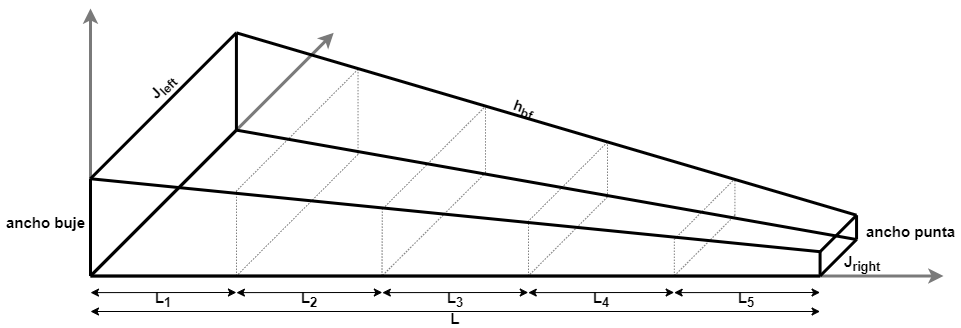
\includegraphics[width=1\textwidth]{images/pala 3d segmentada enorme.png}
    \caption{Representación gráfica de la pala segmentada en 3 dimensiones}
    \label{fig:analisis_volumen}
    \end{figure}

Mediante la observación de la figura \ref{fig:analisis_volumen} se puede obtener la siguiente figura que se usará de análisis para obtener las dimensiones del ancho que se acaba de establecer como tercera dimensión:

    \begin{figure}[H]
    \centering
    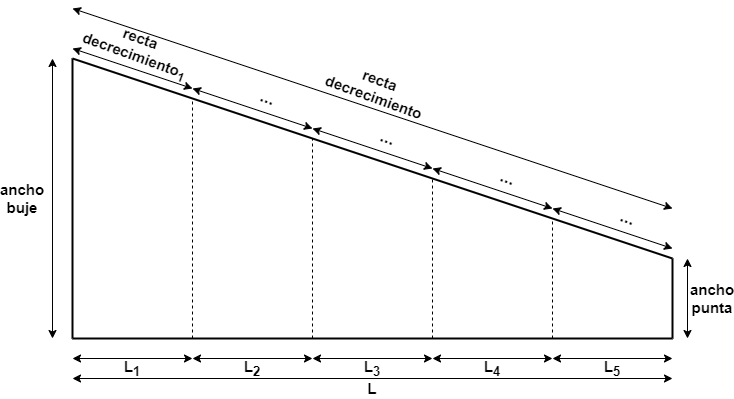
\includegraphics[width=1\textwidth]{images/ancho pala r decrecimiento.png}
    \caption{Representación del ancho de la pala dividida en segmentos}
    \label{fig:ancho_pala_segmentado}
    \end{figure}







\newpage
De la Figura \ref{fig:ancho_pala_segmentado} e imitando el proceso deductivo realizado en la obtención de la Ecuación \ref{def_hipotenusa_pala} se deduce:
\begin{equation}
recta \text{ } decrecimiento_i = \dfrac{( i \cdot \sqrt{L^2 + (ancho \text{ } punta - ancho \text{ } buje)^2)}}{N} \hspace{7pt} (m)
\end{equation}

Siendo, $ancho \text{ } buje$ y $ancho  \text{ } punta$ $\in \mathbb{Q+}$, $ancho \text{ } buje > ancho \text{ } punta$, $recta \text{ } decrecimiento_i $ es la línea de disminución de la parte superior ancho de la pala dividida para cada segmento,  $ancho \text{ } punta$ es la amplitud de la pala del aerogenerador en la zona más estrecha o punta y $ancho \text{ } buje$ es la amplitud de la pala del aerogenerador en la zona más ancha o buje.\\


Tal y como se presentó en la Figura \ref{fig:pala_calculo_phi}, la variable $x_i$ sirvió de apoyo para calcular las reducciones de tamaño de las líneas de cuerda al ir restando el resultado a la variable $c_{left_i}$. Esto mismo ocurre para el ancho de la pala. En esta ocasión además, se necesitará una segunda variable.\\


Las variables de apoyo son las siguientes:
\begin{equation}
 z_i = \sqrt{ recta \text{ } decrecimiento_i^2 - (L_i \cdot i )^2} \hspace{7pt} (m)
 \end{equation}
 \begin{equation}
 b_i =  \left\{\begin{matrix}
0 \hspace{33pt} Sí \hspace{7pt} i = 1\\ 
z_i  \hspace{30pt} Sí \hspace{7pt}  i > 1
\end{matrix}\right
\end{equation}

Donde $z_i$ es la variable de apoyo para el cálculo del área de las secciones trapezoides correspondientes al corte de los segmentos, en este caso de las bases menores y  $b_i$ es la segunda variable de apoyo pero destinada a las bases mayores.\\


Se obtiene el ancho de las bases de los troncos trapezoidales y se calculan las áreas de las bases:
\begin{equation}
 ancho \text{ } base \text{ } menor_i = ancho \text{ } buje - z_i \hspace{7pt} (m)
 \end{equation}
 \begin{equation}
 ancho \text{ } base \text{ } mayor_i = ancho \text{ } buje - b_i \hspace{7pt} (m)
\end{equation}
\begin{equation}
 area \text{ } base \text{ } menor_i = ancho \text{ } base \text{ } menor_i \cdot {c_{right}}_i \hspace{7pt} (m^2)
 \end{equation}
\begin{equation}
 area \text{ } base \text{ } mayor_i = ancho \text{ } base \text{ } mayor_i \cdot {c_{left}}_i \hspace{7pt} (m^2)
\end{equation}

Donde $ancho \text{ } base \text{ } mayor_i$ es el ancho de las bases trapezoidales de mayor tamaño con las que se calculará el volumen del tronco o frustum de cada uno de los segmentos,  $ancho \text{ } base \text{ } menor_i$ es el ancho de las bases trapezoidales de menor tamaño con las que se calculará el volumen del tronco o frustum de cada uno de los segmentos, $ area \text{ } base \text{ } mayor_i $ se refiere a las zonas trapezoidales que sirven de base mayor para el cálculo del frustum de cada segmento y $ area \text{ } base \text{ } menor_i $ se refiere a las zonas trapezoidales que sirven de base menor para el cálculo del frustum de cada segmento.\\


Con todo lo necesario para el cálculo del volumen de la pala del aerogenerador se procede a ello. Se va a realizar de dos maneras; completo y segmentado. El segmentado es necesario debido al desarrollo que se ha ido realizando y que se va a seguir durante todo el trabajo, y el completo se usará para comparación y demostración junto al segmentado para comprobar la precisión de los cálculos.\\

El volumen de la pala de una turbina eólica es definido mediante las siguientes ecuaciones:
\begin{equation}
    \begin{split}
        volumen \text{ } frustum_i = & \dfrac{L_i}{3} \cdot (area \text{ } base \text{ } mayor_i + area \text{ } base \text{ } menor_i \\
        & + \sqrt{area \text{ } base \text{ } mayor_i \cdot area \text{ } base \text{ } menor_i}) \hspace{7pt} (m^3)
    \end{split}
\end{equation}

\begin{equation}
 volumen \text{ } frustum_{total} = \sum_{i}^{N}volumen \text{ } frustum_i \hspace{7pt} (m^3)
\end{equation}

\begin{equation}
 area \text{ } base_{punta} = ancho \text{ } punta * J_{right} \hspace{7pt} (m^2)
 \end{equation}

 \begin{equation}
 area \text{ } base_{buje} = ancho \text{ } buje * J_{left} \hspace{7pt} (m^2)
 \end{equation}
 
 \begin{equation}
    \begin{split}
        volumen \text{ } frustum_{completo} = & \dfrac{L}{3} \cdot ( area \text{ } base_{punta} + area \text{ }  base_{buje}\\
        & + \sqrt{area \text{ } base_{punta} \cdot area \text{ } base_{buje}}) \hspace{7pt} (m^3) 
    \end{split}
 \end{equation}

Donde $ volumen \text{ } frustum_i $ es el tamaño de cada uno de los segmentos del tronco de pirámide de la pala del aerogenerador, $ volumen \text{ } frustum_{total} $ es el tamaño absoluto de la pala del aerogenerador, $area \text{ } base_{punta}$ es la zona trapezoidal de mayor tamaño usada para el cálculo del volumen del frustum, $area \text{ } base_{punta}$ es la zona trapezoidal de menor tamaño usada para el cálculo del volumen del frustum y $ volumen \text{ } frustum_{completo} $ es el tamaño integro de la pala del aerogenerador.\\


Teniendo los cálculos del volumen de la pala del aerogenerador se pueden estudiar a continuación los efectos que producen las simplificaciones que se han realizado para la obtención de energía.


\subsection{Estudio del torque sin ángulo de cabeceo}
\label{section:no_cabeceo}

Tomando una pala con forma real, en una situación en la que no se presenta cabeceo, en la que está incidiendo un viento con ángulo de ataque paralelo a la pala se puede observar un giro de las palas del aerogenerador.\\

Al estar la pala real más redondeada por la parte superior y teniendo mayor volumen que la parte inferior y mediante el principio de Bernoulli la parte superior presenta un mayor recorrido que la inferior, y con ello una velocidad de viento mayor y por tanto una menor presión. \\

Este efecto produce un gradiente de presión y por ello una fuerza de sustentación. Debido la no simetría de las palas del aerogenerador como se muestra en la Figura \ref{fig:corte_transversal_pala}. \\

    \begin{figure}[H]
    \centering
    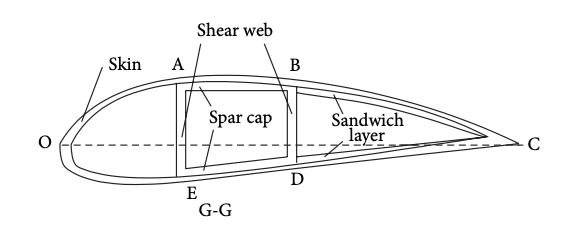
\includegraphics[width=0.8\textwidth]{images/Cross secction pala articulo.png}
    \caption{Corte transversal de una pala}
    Fuente: \cite{Zheng2014}
    \label{fig:corte_transversal_pala}
    \end{figure}


% Debido a este fenómeno se va a trabajar con una pala simplificada (ver la Figura \ref{fig:analisis_volumen}) que simplificará cálculos. \\



\subsection{Estudio del torque con ángulo de cabeceo}
\label{section:torque_giro_inicial}

El ángulo $ \theta_1 $ es el \textit{ángulo de cabeceo} que sufrirán todos y cada uno de los segmentos que son paralelos al plano horizontal, desde el cual se presenta el viento que incidirá en la pala.\\


En esta sección se estudiará qué ocurre en término de fuerzas, torque y momento cuando se gira toda la pala únicamente el ángulo de cabeceo $ \theta_1 $. \\


Al inclinar odos los segmentos un ángulo $ \theta_1 $ se genera la situación en la que el viento incide en el centro del segmento con el mismo ángulo con el que se inclina la pala (ver Figura \ref{fig:dibujo_fuerzas}). \\

\begin{figure}[H]
    \centering
    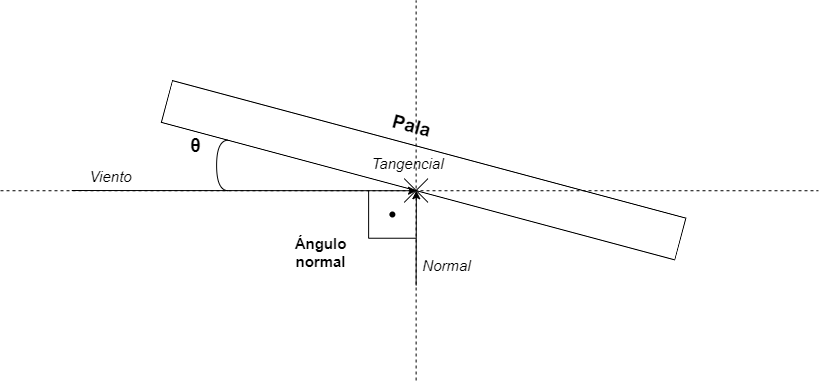
\includegraphics[width=1\textwidth]{images/dibujo fuerzas.drawio.png}
    \caption{Ángulo de ataque del viento con respecto a la pala y descomposición de vectores de fuerzas}
    
    \label{fig:dibujo_fuerzas}
\end{figure}

La fuerza del viento que incide en la pala se puede descomponer en dos, la tangencial y la normal. El vector fuerza normal es perpendicular al ángulo de ataque del viento, mientras que el vector fuerza tangencial recorre de manera paralela la línea central de la pala.\\

 La fuerza normal viene definida por la siguiente expresión:
 \begin{equation}
   f \text{ } normal = F \text{ } viento \cdot \sin{\theta_1} \hspace{7pt} (N)
 \label{def:fuerza_normal}
 \end{equation}
 Donde $F \text{ } viento$ es la fuerza generada por el viento en cada segmento de la pala y $f \text{ } normal$ es la fuerza perpendicular al viento, generada por el choque de este con la pala de la turbina eólica.\\


La componente paralela a la pala, que se ha definido como tangencial se obviará debido a que no genera momento de torsión o torque.\\
  
El momento de giro o torque se define como:
  \begin{equation}
  torque_0 = f \text{ } normal \times brazo \hspace{7pt} (N \cdot m)
  \label{def:torque_inicial}
 \end{equation}
 Donde $torque_0$ := Momento de fuerza de giro solo con ángulo de cabeceo.\\


El $torque_0$ es el producto vectorial entre la $fuerza  \text{ }perpendicular \text{ } o \text{ } normal$ y el $brazo$. Pero estas dos variables son perpendiculares la una a la otra, es por ello que esa expresión es el producto algebraico de las variables, dando lugar a:
 
 
  \begin{equation}
  torque_{0_i} = f \text{ } normal_i \cdot brazo_i \hspace{7pt} (N \cdot m)
 \label{def:torque_algebraico_inicial}
 \end{equation}
 
 La suma de los torques es torque global.
 \begin{equation}
  torque \text{ } global_0 \text{ } = \sum_{i=1}^{N} torque_{0_i} \hspace{7pt} (N \cdot m)
\label{def:torque_global}
\end{equation}
 
 
La fuerza del viento para el rotor completo es:
 \begin{equation}
  F \text{ } viento = \dfrac{1}{2} \text{ } \rho \cdot area \text{ } rotor \cdot u^2 \cdot coeficiente \text{ } sustentación \hspace{7pt} (N)
   \end{equation}
   
    Donde $\rho = 1.225 \text{ } \dfrac{Kg}{m^3}$, $u$ es la velocidad del viento, $area \text{ } rotor$ es la superficie del círculo que dibuja el giro de las palas y $coeficiente \text{ } sustentación$ es el número usado en la modelación y sus dependencias complejas de forma, inclinación y algunas condiciones de flujo en la sustentación \cite{Hall2021}.
    
  \begin{equation}
  area \text{ } rotor = \dfrac{\pi}{4} \cdot diametro \text{ } rotor^2 \hspace{7pt} (m^2) 
  \end{equation}
  Donde $diametro \text{ } rotor $ es la superficie abarcada por la pala en caso de realizar un giro completo
  \begin{equation}
  diametro \text{ } rotor = 2 \cdot L \hspace{7pt} (m)
 \end{equation}

 En la Sección \ref{section:no_cabeceo} se menciona la existencia de una fuerza de sustentación que genera torque cuando el viento incide de manera paralela sobre la pala del aerogenerador.\\
 
 Cuando se introduce un ángulo de cabeceo y debido a la forma de la sección de la pala, Figura \ref{fig:dibujo_fuerzas}, es posible incluir la variable conocida como \textit{coeficiente sustentación}. Este se produce debido a las fuerzas de empuje del viento y su valor es obtenido mediante la siguiente representación:
 
 \begin{figure}[H]
    \centering
    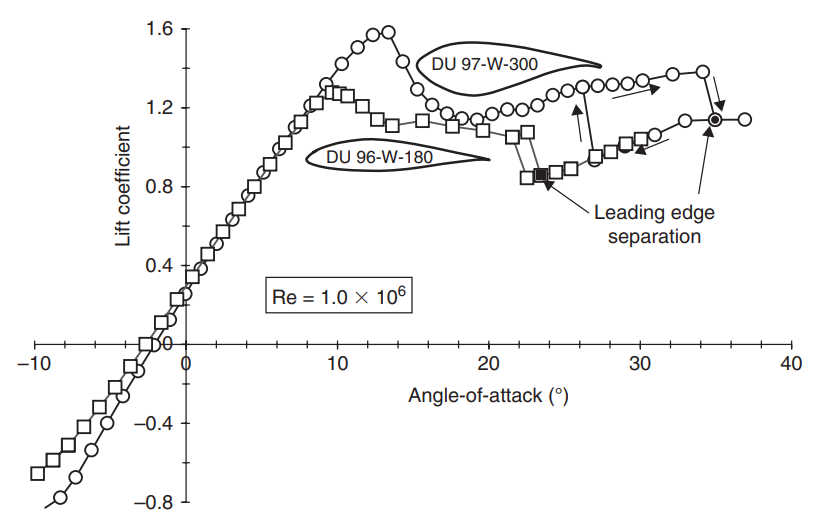
\includegraphics[width=1\textwidth]{images/imagen del coeficiente sustentacion.PNG}
    \caption{Curva de sustentación medida para un aerogenerador que tiene una superficie sustenadora con un espesor de entre 18\% y 25\% }
    Fuente: Artículo \cite{TIMMER2013109}, Figura 4.13
    \label{fig:plot_coef_sustentacion}
\end{figure}



 
 \subsection{Estudio del torque con ángulo de cabeceo y torsión de la pala}
\label{section:torque_giro_torsion}

La única diferencia entre este apartado y el anterior es el ángulo de giro de los segmentos. Anteriormente, se vió como todos los segmentos giraban un determinado \textit{ángulo de cabeceo}, pero ahora el ángulo que se girarán vendrá dado por:

Dados un ángulo inicial de giro $\theta_1 $ y una variación de giro constante (o no) $\Delta_\theta$, se define el ángulo de torsión de cada segmento como:
\begin{equation}
\theta_i = \theta_{i-1} + \Delta_\theta \hspace{7pt} (^{\circ})
\label{def:theta_cte}
\end{equation}
Donde $i \in segmento \wedge (i > 1)$\\


Como se menciona, la variación $\Delta_\theta$ puede que no sea constante y entonces:
\begin{equation}
\theta_i = \theta_{i-1} + \Delta_{\theta_{i}}  \hspace{7pt} (^{\circ})
\label{def:theta_nocte}
\end{equation}
Donde $i \in segmento \wedge (i > 1)$\\

La fuerza normal se define como:
\begin{equation}
   f \text{ } normal_i = F \text{ } viento \cdot \sin{\theta_i} \hspace{7pt} (N)
  \label{def:fuerza_normal_torsion}
 \end{equation}

El resto de fórmulas no varían debido a que no dependen del ángulo $\theta_i$. En el caso del \textit{torque global} la suma de torques nos aportará un conjunto de valores diferentes y que servirán como estudio.

  \begin{equation}
  torque_{1_i} = f \text{ } normal_i \cdot brazo_i \cdot \cos{\Delta_{\theta_{i}}} \hspace{7pt} (N \cdot m)
 \label{def:torque_algebraico_torsion}
 \end{equation}
 
Donde $ \cos{\Delta_{\theta_{i}}} $ puede presentar una pequeña variación en el valor del torque. Este coseno representa el área efectiva donde se está aplicando la $ f \text{ } normal $, es decir, el área de la totalidad del segmento de la pala si fuera observada desde arriba en un plano XY. Esto se debe a que cuanto más se torsione el segmento, menos parte será visible.\\

Por último, la suma de los torques con un giro inicial es entonces:
\begin{equation}
  torque \text{ } global_1 \text{ } = \sum_{i=1}^{N} torque_{1_i} \hspace{7pt} (N \cdot m)
 \label{def:torque_global_1}
\end{equation}
Donde $torque \text{ } global_1$ es la suma de torque de los N segmentos.





















\subsection{Cálculo de la potencia del sistema}
\label{section:pot_sistema}
 
 \textcolor{orange}{\huge La potencia depende de la turbina con la que estés trabajando, y del tamaño de las palas.}
 
 Una vez se tiene todo lo necesario para el cálculo del torque, se puede pasar al cálculo de la potencia. Esta es la variable más importante, cuanta mayor cantidad de energía se genere, mejor, aunque existe un límite directamente relacionado con las limitaciones técnicas y físicas que presentan las turbinas eólicas. \\
 
 
  La potencia del sistema con un ángulo de cabeceo se define como:
  \begin{equation}
  potencia \text{ } global_0 = torque \text{ } global_0 \cdot \Omega  
 \label{def:potencia_giro_inicial}
 \end{equation}
  Donde $\Omega$ := velocidad de giro o angular de la pala y $potencia \text{ } global_0$ := energía del sistema.\\
 
  La potencia del sistema con un giro inicial y torsión se define como:
   \begin{equation}
  potencia \text{ } global_1 = torque \text{ } global_1 \cdot \Omega  
 \label{def:potencia_giro_segmentos}
 \end{equation}
  Donde $potencia \text{ } global_1$ := Energía del sistema con un cierto ángulo de cabeceo y segmentos torsionados.\\
 
Las unidades que se buscan serían, la potencia en $W$ ($Watts$) o $\dfrac{J}{s}$ ($\dfrac{Julio}{segundo}$) porque el torque es en $\dfrac{N}{m}$ ($\dfrac{Newton}{metro}$) o $J$ y $\Omega$ en $\dfrac{1}{s}$ o $s^{-1}$.

 
\subsection{Momento de inercia general de los segmentos de la pala}

Para poder calcular la $\Omega$ es necesario obtener el momento de inercia.\\

En \cite[p.~269]{goldstein1987mecanica} se define el $momento \text{ } de \text{ } inercia$ respecto a un eje como la suma, extendida a todas las partículas del cuerpo, del producto de la masa de cada partícula por el cuadrado de su distancia al eje.\\


La geometría del cuerpo libre que está realizando la rotación es crucial, por ello dependiendo de esta, el cálculo del momento de inercia variará. En \cite[p.~242]{oberg2012machinery} se encuentra el momento de inercia de un trapecio. \\


\begin{figure}[H]
    \centering
    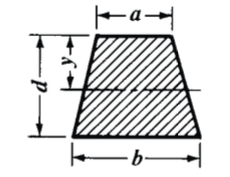
\includegraphics[width=0.3\textwidth]{images/trapecio libro machinery.png}
    \caption{Sección trapezoidal}
    Fuente: \cite[p.~242]{oberg2012machinery}
    \label{fig:momento_inercia_libro}
\end{figure}



\begin{equation}
    I = \dfrac{ d^3 \cdot (a^2 + 4 \cdot a \cdot b + b^2)}{ 36 (a + b)} \hspace{7pt} (m^4) 
\end{equation}




El momento de inercia generalmente se calcula mediante la posición del centro de masa. Pero las figuras que giran en un eje, no siempre lo hacen con respecto al eje perpendicular que atraviesa el centro de masa, en ocasiones el eje de giro se encuentra fuera de la figura, en ese caso se aplica el $Teorema \text{ } de \text{ } Huygens-Steiner$ o $Teorema \text{ } del \text{ } eje \text{ } paralelo$. \\

Este teorema establece que se puede calcular el momento de inercia de un cuerpo rígido en cualquier eje paralelo al que pasa atravesando a la figura por el centro de masas. Para ello es necesario conocer la distancia perpendicular entre los ejes paralelos (que se definió anteriormente como $brazo$) y la masa del cuerpo, que en nuestro caso será la masa de cada segmento. \\

El teorema de Huygens-Steiner establece lo siguiente:
 \begin{equation}
    I = I_{cm} + m \cdot D^2 \hspace{7pt} (Kg \cdot m^2)
 \label{eq:Huygens-Steiner}
 \end{equation}
 Donde $I$ es el momento de inercia general, $I_{cm}$ es el momento de inercia en el centro de masas de un cuerpo rígido, $m$ es la masa del cuerpo rígido y $D$ es la distancia perpendicular entre los ejes paralelos.\\\\
 

Si se combina la Ecuación \ref{eq:Huygens-Steiner} junto con las variables definidas para el estudio de la pala el momento de inercia vendrá dado por la siguiente definición:
 \begin{equation}
  I_{area_i} = \dfrac{ L_{i}^3 \cdot (c_{right}^2 + 4 c_{right} \cdot c_{left} + c_{left}^2)}{ 36 (c_{right} + c_{left})} \hspace{7pt} (m^4)
 \label{def:momento_inercia_area}
 \end{equation}
 Donde $I_{area}$ es el momento de inercia de área de una figura de un espesor mínimo para centrar su cálculo en la forma.\\
 
 La anterior ecuación se debe multiplicar por la \textbf{densidad superficial} de la pala del aerogenerador ya que esta representa el momento de inercia de un área, en este caso un trapecio, y se necesita esta densidad para obtener el momento de inercia general.\\

En el cálculo de la \textbf{densidad superficial} son necesarios dos términos que aún no se han acuñado en este trabajo, la masa y la superficie de una pala. Es cierto que se ha calculado la superficie de los segmentos en la Definición \ref{def:area_segmentos}, ahora solo queda sumarlos.\\


La superficie de la pala es:
 \begin{equation}
 superficie \text{ } pala = \sum_{i}^{N}s_i \hspace{7pt} (m^2)  
 \label{def:superficie_pala}
 \end{equation}
  Donde $ superficie \text{ } pala $ es el área de la pala del rotor.\\

En este trabajo solo se han tenido en cuenta los tres materiales mas usados en la construcción de palas de un aerogenerador.\\

Los rangos de densidades de materiales \cite{MOHAMMED201969} \cite{Tewari2011} \cite{Ephraim2015} utilizadas son los siguientes:
 \begin{equation}
 densidad \text{ } pala =  \left\{\begin{matrix}
CFRP = 1500-2000 \hspace{7pt} \left(\dfrac{Kg}{m^3}\right) \\\\
GFRP = 910-1200 \hspace{7pt} \left(\dfrac{Kg}{m^3}\right)  \\\\
GF \text{ } Epoxy = 1159-1186 \hspace{7pt} \left(\dfrac{Kg}{m^3}\right) 
\end{matrix}\right
\label{def:materiales_pala}
\end{equation}
 Donde $ densidad \text{ } pala $ es la densidad de los materiales de los que posiblemente esté compuesta la pala, $ CFRP $ sin abreviatura carbon fiber reinforced polymer o en castellano; polímero reforzado con fibra de carbono, $ GFRP $ sin abreviatura glass fiber reinforced polymer o en castellano; polímero reforzado con fibra de vidrio y $GF \text{ } Epoxy $ sin abreviatura glass fiber reinforced Epoxy o en castellano; Epoxy reforzado con fibra de vidrio.\\

Parte de la pala es hueca. Existen estudios \cite{Pourrajabian2016} en los cuales se compara el uso de palas compactas y huecas en determinado escenario y con diferentes grosores de material. \\

En este trabajo, las palas serán huecas y se estima que solo entre un $15-20\%$ de la pala presenta alguno de los materiales que se mencionan. Por ello la expresión de la masa es la siguiente. \\

La masa de los segmentos de una pala dada su densidad y volumen:
 \begin{equation}
 masa \text{ } pala = densidad \text{ } pala \cdot (volumen \text{ } frustum_{total} \cdot (15-20\%) ) \hspace{7pt} (Kg)
 \end{equation}
 \begin{equation}
 masa \text{ } segmento_i = \dfrac{s_i}{superficie \text{ } pala} \cdot masa \text{ } pala \hspace{7pt} (Kg)
 \label{def:masa_pala} 
 \end{equation}
  Donde $ masa \text{ } pala $ es el peso de la aleta de la turbina eólica teniendo en cuenta la porción no rellena de la misma y $ masa \text{ } segmento_i $ es el peso de los segmentos de la aleta.\\
 
 
Se puede pasar a calcular la $densidad \text{ } superficial$ como:
  \begin{equation}
 densidad \text{ } superficial = \dfrac{masa \text{ } pala}{ superficie \text{ } pala} \hspace{7pt} \left(\dfrac{Kg}{m^2}\right)
 \label{def:densidad_superficial}
 \end{equation}
 Donde $ densidad \text{ } superficial $ generalmente se define como masa de un material por unidad de superficie. \\
 
 
  \colorbox{orange}{¿Es correcto multiplicarlo por la densidad superficial? Con carlos hablé de thickness, pero está en metros}
 
Se puede obtener el momento de inercia general o $I_i$ mediante el Teorema \ref{eq:Huygens-Steiner}, como:
  \begin{equation}
I_{cm_i} = I_{area_i} \cdot densidad \text{ } superficial \hspace{7pt} (Kg \cdot m^2)
 \label{def:momento_inercia_cm}
 \end{equation}
 \begin{equation}
I_i = I_{cm_i} + masa \text{ } segmento_i \cdot brazo_i^2 \hspace{7pt} (Kg \cdot m^2)
 \label{def:momento_inercia_general}
 \end{equation}

 
\subsection{Velocidad Angular, $\Omega$, en función de la velocidad del viento }

En primer lugar, la velocidad angular $\Omega$ se define como ``la componente de un vector unidimensional a lo largo del eje de rotación en relación con el sistema de coordenadas elegido para describir el movimiento'' \cite[p.~303]{cummings2004understanding}.\\

Aplicando la anterior definición al sistema que se está estudiando se se tiene que el rotor del aerogenerador sería el eje de rotación en base al cual giran las palas de la turbina. Además el movimiento de giro es constante alrededor del rotor.\\

Una de las opciones más sencillas para el cálculo de la \textit{velocidad angular} es mediante la aceleración angular y la relación que tiene con el \textit{torque} y con el \textit{momento de inercia general}. Pero no era lo suficientemente preciso y no tenía en cuenta todos los aspectos de la cinemática. \\
 
Para que el sistema se encuentre girando a una cierta \textit{velocidad angular} primero se debe producir una cierta \textit{aceleración angular}, producida por el viento. Con el viento y otros factores el rozamiento del aire, el peso de las palas y la fuerza necesaria para moverlas, se podría llegar a mantener una velocidad de giro óptima y así extraer la mayor cantidad de energía. Pero la velocidad del viento es aleatoria, aunque se considera su valor medio como constante.\\


Una de las partes fundamentales es el viento que se presenta delante de la turbina y su velocidad, es decir, la masa o flujo de aire que atravesará el rotor de la turbina. En este caso del aire se obtendrá mediante la relación del volumen frente a la turbina y la densidad del mismo, que puede variar dependiendo de las condiciones meteorológicas.\\

La masa de aire con la que trabaja el rotor es:
\begin{equation}
    masa \text{ } aire = volumen \text{ } rotor \cdot \rho \hspace{7pt} (Kg)
\label{def:masa_aire}
\end{equation}
\begin{equation}
    volumen \text{ } rotor = \dfrac{\pi}{4} \cdot diametro \text{ } rotor^2 \cdot J_{left} \hspace{7pt} (m^3) 
\end{equation}
\begin{equation}
     diametro \text{ } rotor = 2L + diametro \text{ } gondola \hspace{7pt} (m)
\end{equation}
Donde \textit{diametro rotor} es el ancho total del rotor sumando palas y góndola, \textit{diametro gondola} es el ancho de la góndola del rotor, \textit{volumen rotor} es el tamaño de la figura dibujada (cilindro) por el rotor completo cuando las palas giran y \textit{masa aire} es el peso del aire comprendido dentro del volumen que define el rotor.\\

La energía cinética producida por la masa de aire que comprende el rotor y la velocidad del viento en ese momento es:
\begin{equation}
    E_c = \dfrac{1}{2} \cdot masa \text{ } aire \cdot u^2 \hspace{7pt} (J)
\end{equation}
Donde $E_c$ es la energía generada por el movimiento de las palas del rotor.\\


A continuación se introduce un término que limita la energía cinética que se puede obtener en un aerogenerador, se trata del \textit{coeficiente de potencia} $CP$.\\

El valor máximo de esta variable adimensional es 0.593, este valor se conoce como Límite de Betz. Albert Betz establece que el límite máximo de aprovechamiento de energía cinética que se puede obtener de la energía del viento es el 59.3\%. Este realizó un experimento en el cual define un tubo de corriente con condiciones ideales dentro del cual se encuentran las palas de la turbina eólica, estas al girar obtienen energía, pero también generan bloqueos y turbulencias con el viento que las atraviesa. Estas dos hacen que que el tubo de corriente se ensanche y se pierda velocidad del viento en la estela de la turbina \cite{NEILL201883}.\\


En la figura, la flecha indica la dirección del viento y también se observa la expansión de la estela.

\begin{figure}[H]
    \centering
    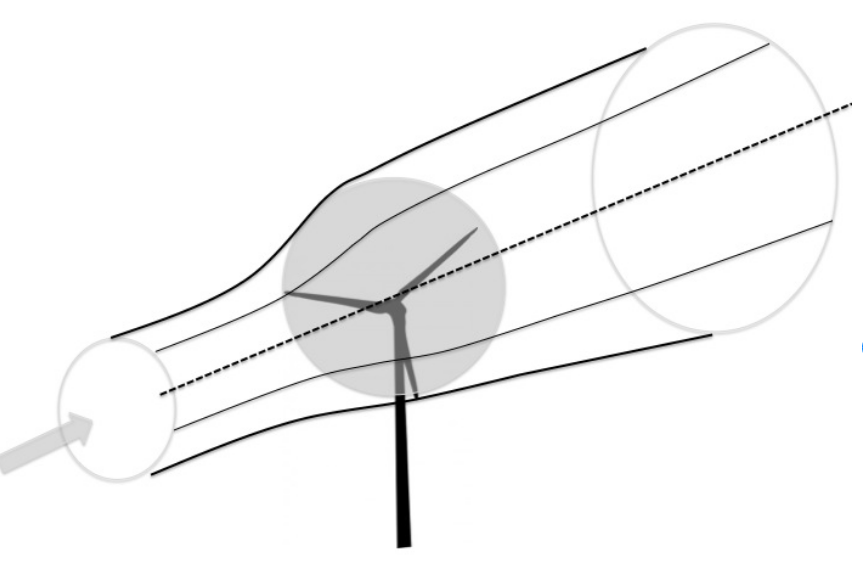
\includegraphics[width=0.8\textwidth]{images/Figura articulo Modelling Smart Wind Turbine Blades.PNG}
    \caption{Tubo de corriente producido por un aerogenerador}
    Fuente: Tesis \cite{Vinit2015}, Figura 2.1
    \label{fig:Tubo_corriente_betz}
\end{figure}


La derivada de la potencia extraída entre la potencia del viento en el tubo de flujo que se definió da como resultado el \textit{límite de Betz}.\\


Al introducir este término en la ecuación anterior, se pasa de tener una energía cinética simple a una aprovechada o de rotación.\\




\begin{equation}
    E_c \text{ } aprovechada = E_c \cdot CP \hspace{7pt} (J)
\end{equation}
Donde $E_c \text{ } aprovechada$ es la energía máxima generada por el movimiento de las palas del rotor teniendo en cuenta las limitaciones técnicas del aerogenerador.\\

Se presenta la segunda manera de obtener la energía cinética de rotación:
\begin{equation}
    E_c  \text{ } rotacion = \dfrac{1}{2} \cdot I_i \cdot \Omega^2  \hspace{7pt} (J)
\end{equation}
Donde $E_c \text{ } rotacion$ es la energía que se produce mediante el giro producido por el momento de inercia general y la velocidad angular de los segmentos de la pala. \\

Se comparan las dos energías cinéticas y se obtiene la velocidad angular para cada segmento de la pala:
\begin{equation}
    \Omega_i = \sqrt{\dfrac{CP \cdot M_{aire}}{I_i}} \cdot u  \hspace{7pt} (\dfrac{rad}{s})
\end{equation}


 \subsection{Rendimiento de la turbina}
 \label{section:rendimiento}
 
La comparación de potencias da como resultado un rendimiento, este permite determinar si la torsión de la pala genera una variación en la potencia obtenida.\\

El rendimiento del sistema viene definido por:
\begin{equation}
  \eta = \dfrac{potencia \text{ } global_1}{potencia \text{ } global_0}  
 \label{def:rendimiento_potencias}
 \end{equation}
  Donde $\eta$ := eficiencia respecto a la energía obtenida en dos casos estudiados.\\
 
 Una vez definido el rendimiento, se calcula en base a los resultados obtenidos mediante asignación de valores a variables estándar se pueden dar 3 escenarios:
 

\begin{enumerate}
    \item $\eta < 1$
        \begin{itemize}
            \item En caso de obtener un valor por debajo de 1, quiere decir que la torsión que se aplicó, ha reducido la obtención de energía con respecto al caso base. 
        \end{itemize}
    \item $\eta ~= 1$
        \begin{itemize}
            \item Si el valor obtenido es muy próximo a 1, entonces el caso base y el estudiado proporcionan valores similares de obtención de energía.
        \end{itemize}
    \item $\eta > 1$
        \begin{itemize}
            \item Este es el valor buscado y el objetivo del estudio, que una pala con torsión obtenga más energía que una sin ello.
        \end{itemize}
\end{enumerate}

Cabe recalcar que se deberán hacer numerosas pruebas con diferentes configuraciones de valores de las principales variables que definen la pala y los aspectos físicos que afectan a la generación de energía.